\documentclass[review]{elsarticle}
\usepackage{amsmath,amssymb}
\usepackage{latexsym}
\usepackage{booktabs}
%% Packages
\usepackage{geometry}
\usepackage{amsthm}
\usepackage{stmaryrd}
\usepackage{graphicx}
\usepackage[singlespacing]{setspace}
\usepackage{float}
\usepackage{endnotes}
\setcounter{MaxMatrixCols}{20} 
\usepackage{indentfirst}
\usepackage{geometry}
\usepackage{subfig}

\usepackage{latexsym}
\usepackage{booktabs}
\usepackage{geometry}
\usepackage{amsthm}
\usepackage{stmaryrd}

\usepackage{subfig}
\usepackage{color}
\usepackage[export]{adjustbox}
\usepackage{listings}
\usepackage{epstopdf} 
\lstset{language=Matlab}
\lstset{breaklines}
\lstset{extendedchars=false}

\usepackage{mathtools}
\usepackage[ruled,linesnumbered]{algorithm2e}
\DeclarePairedDelimiter\ceil{\lceil}{\rceil}
\DeclarePairedDelimiter\floor{\lfloor}{\rfloor}
\usepackage{graphicx}
\usepackage{epstopdf}
\usepackage{multirow}
\usepackage{paralist}
\usepackage{amsmath,amsthm,amssymb}
\usepackage{setspace}
\usepackage{float}
\usepackage{morefloats}
\usepackage[]{algorithm2e}
\usepackage{mdwlist}
\usepackage{booktabs} % FvW: makes tables look nicer
\usepackage{amsfonts}
\usepackage{paralist}
\newcommand{\be}{\begin{equation}}
\newcommand{\ee}{\end{equation}}

\theoremstyle{plain}
\newtheorem{theorem}{Theorem}[section]
\newtheorem{corollary}{Corollary}[section]
\newtheorem{lemma}[theorem]{Lemma}
\newtheorem{proposition}[theorem]{Proposition}
\newtheorem{defn}{Definition}[section]
\newtheorem*{theoremA}{Theorem}
\newtheorem*{theoremB}{Theorem}
\usepackage{pifont}
\theoremstyle{definition}
\newtheorem{assumption}[theorem]{Assumption}
\newtheorem{example}[theorem]{Example}
\newcommand{\RNum}[1]{\uppercase\expandafter{\romannumeral #1\relax}}
\theoremstyle{remark}
\newtheorem*{claim}{Claim}
\usepackage{lineno,hyperref}
\modulolinenumbers[5]
\usepackage{geometry}
\usepackage{subfig}
\usepackage{color}
\usepackage[export]{adjustbox}
\usepackage{listings}
\usepackage{epstopdf} 
\lstset{language=Matlab}
\lstset{breaklines}
\lstset{extendedchars=false}
\geometry{verbose,letterpaper,tmargin=1in,bmargin=1in,lmargin=1in,rmargin=1in}

%% Equation numbering
\numberwithin{equation}{section}
% Users of the {thebibliography} environment or BibTeX should use the
% scicite.sty package, downloadable from *Science* at
% www.sciencemag.org/about/authors/prep/TeX_help/ .
% This package should properly format in-text
% reference calls and reference-list numbers.
\journal{Transportation Research Part *}

% If your reference list includes text notes as well as references,
% include the following line; otherwise, comment it out.

\bibliographystyle{elsarticle-num}
% CAPTIONS

%% Allow display breaks
\allowdisplaybreaks

\newtheorem{remark}[theorem]{Remark}
\theoremstyle{remark}
\renewcommand{\thesubsubsection}{\arabic{subsubsection}.}
%% Paragraph spacing
\setlength{\parskip}{1ex}

%% Redefine maketitle
\makeatletter

\makeatother
\begin{document}
	
\begin{frontmatter}
	
	\title{Modeling the spreading of infectious disease through transportation network}
	
	%% Group authors per affiliation:
	\author[mymainaddress]{Xinwu Qian}
	\ead{qian39@purdue.edu}
	
	
	%% or include affiliations in footnotes:
	\author[mymainaddress]{Satish V. Ukkusuri}
	\cortext[mycorrespondingauthor]{Satish V. Ukkusuri}
	\ead{sukkusur@purdue.edu}

	
	\address[mymainaddress]{Lyles school of Civil Engineering, Purdue University, West Lafayette, IN 47907, USA}

\begin{abstract}
The rapid urbanization in the past few decades brings billions of people into urban areas. The process generates multiple mega-cities around the world with intensive activities, which contributes to the boost of economy. However, these cities are vulnerable to outside attacks such as diseases due to enormous population size and activity density. The leading cause for the spread of infectious diseases is human contagion, which is driven by the mobility provided from the urban transportation system. In this project, we investigate preventing infectious diseases by controlling the mobility of urban transportation system. In particular, the spread of disease is formulated as bilinear S-E-I-R system, and different levels of control on urban transportation system are modeled as a hybrid system. The objective is to understand if controlling urban transportation system may help to eliminate or reduce the speed of disease spreading by properly designing the hybrid system.
\end{abstract}
	
	\begin{keyword}
		\texttt{Disease modeling} \sep traffic network \sep reachable set  
		\MSC[2017] 00-01\sep  99-00
	\end{keyword}
	
\end{frontmatter}

\linenumbers
\section{Introduction}

Add introduction part with literature review here. 
\newpage
\section{Notation}
The table of notation is presented in Table~\ref{notation}.
\begin{table}[h]
	\setstretch{1.2}
	\centering
	\caption{Table of notation}
	\label{notation}
	\begin{tabular}{p{3cm}p{13cm}}
		\hline
		Notation & Description \\ \hline
		&\textbf{Variables}\\ \hline
		$S_i$ & Susceptible population at patch $i$. \\
		$E_i$ & Exposed (latent) population at patch $i$.\\
		$I_i$ & Infected population at patch $i$. \\
		$R_i$ & The population who recovered from disease and got immunity at patch $i$.\\
		$S_{ij}^m$ & The susceptible population who travel from patch $i$ to patch $j$ using mode $m$. \\
		$E_{ij}^m$ & The exposed population who travel from patch $i$ to patch $j$ using mode $m$. \\
		$I_{ij}^m$ & The infected population who travel from patch $i$ to patch $j$ using mode $m$. \\
		$t_{ij}^m$ & Induced travel time for moving from patch $i$ to patch $j$ using mode $m$. \\
		$N_i^p$ & Population at patch $i$. \\
		$N_{ij}$ & The amount of people currently at patch $j$ who are the residents of patch $i$. \\
		\hline
		&\textbf{Fixed parameters}\\ \hline
        $n$ & number of zones in the area. \\
		$\beta_{inn}$ & Within zone contact rate. \\
		$\beta_{tra}^m$ & Contact rate in travel mode. $m$ \\ 
		$1/\sigma $ & Average length of lament period. \\
		$1/\gamma $ & Average length of infected period.\\
		$g_i$ & Total departure rate of patch $i$.\\
		$m_{ij}$ & The rate of movement from path $i$ to path $j$, where $\sum_j m_{ij}=1$. \\
		$c_{ij}^m$ & The ratio of people who choose travel mode $m$ between patch $i$ and patch $j$. \\
		$d_l^m$ & Rate of remaining infected people for travel mode $m$ at control level $l$. \\
		$N_i^r$ & Number of residents at patch $i$. \\ \hline
	\end{tabular}
\end{table}
\section{Disease Dynamics}
In 1927, W.O.Kermack and A.G.McKendrick created a model in which they considered a fixed population with only three compartments: susceptible, $S(t)$, infected, $I(t)$ and removed, $R(t)$. They are defined as follow \cite{kermack1927contribution}:

\begin{itemize}

\item $S(t)$ is used to represent the number of individuals not yet infected with the disease at time t, or those susceptible to the disease.
\item $I(t)$ denotes the number of individuals who have been infected with the disease and are capable of spreading the disease to those in the susceptible category.
\item $R(t)$ is the compartment used for those individuals who have been infected and then removed from the disease, either due to immunization or due to death. Those in this category are not able to be infected again or to transmit the infection to others.
 
\end{itemize}

Several assumptions were made in the formulation of these equations: First, an individual in the population must be considered as having an equal probability as every other individual of contracting the disease with a rate of $\beta$.  For the second and third equations, consider the population leaving the susceptible class as equal to the number entering the infected class. And $\gamma$ represents the mean recovery/death rate, or $1/\gamma$ the mean infective period of infectives are leaving this class per unit time to enter the removed class. Moreover, assuming a death rate $\mu$ and birth rate equal to death rate.\\

Based on the SIR model, the SEIR model was later studied by introducing the latent class (E) \cite{lloyd1996spatial}. Since the SIR model discussed above takes into account only those diseases which cause an individual to be able to infect others immediately upon their infection. However, many diseases have what is termed a latent or exposed phase, d6uring which the individual is said to be infected but not infectious. Thus, a fourth term denoted by $E(t)$ is introduced to represent the number of exposed individuals in the SEIR model. Using a fixed population, $N=S(t)+E(t)+I(t)+R(t)$ and assuming the mean latent period of the disease is $1/\sigma$, the following equations can be obtained:

\begin{eqnarray}
&&\frac{dS}{dt}=-\beta SI+\mu (N-S) \\ \nonumber
\\ 
&&\frac{dI}{dt}=\sigma E-\gamma I-\mu I\\ \nonumber
\\
&&\frac{dE}{dt}=\beta SI-\mu E-\sigma E\\ \nonumber
\\ 
&&\frac{dR}{dt}=\gamma I-\mu R 
\end{eqnarray}

It can be observed that if the latent period tends to zero, corresponding to $\sigma \rightarrow \infty$, there will not be any individuals in the exposed class, and the SEIR model reduces to the SIR model.

\section{Mobility model}
For the $P$ patches of a city, we can write the following two flow conservation equations regarding the movement of people around the city:
\begin{equation}
N_i^r=\sum_{j=1}^{P} N_{ij}
\end{equation}
\begin{equation}
N_i^p=\sum_{j=1}^P N_{ji}
\end{equation}
The first equation suggests that the amount of residents at patch $i$ can be calculated as the summation of population who are residents of  patch $i$ and currently at patch $j$. Similarly, the second equation states that the total population at patch $i$ consists of the residents of patch $i$ who remain in $i$, as well as the population who reach patch $i$ from other patches.

 
Moreover, we introduce the following equations to characterize the dynamics of population flow across the city (for the following part, let $\dot{K}$ denotes the time derivative $\frac{dK}{dt}$ ):
\begin{equation}
\dot{N}_{ij}=-r_{ij}N_{ij}+g_im_{ij}N_{ii}
\end{equation}
\begin{equation}
\dot{N}_{ii}=\sum_{j=1}^P r_{ij}N_{ij}-g_iN_{ii}
\end{equation}
It can be observed from the first equation that there are two components affecting the amount of people who are residents of $i$ and currently at $j$: the rate that people return to patch $i$ and the rate that new travelers from patch $i$ arrives in $j$. As for $N_{ii}$, the change in population is measured by the difference between the return of residents from all other patches and the total amount of residents departed. Based on the two ordinary differential equations (ODEs), we arrive at the following two ODEs which quantify the dynamics of the amount of residents and population:
\begin{equation}
\dot{N}_i^r=\sum_{j=1}^P \dot{N}_{ij}=\sum_{j=1}^P r_{ij}N_{ij}-g_iN_{ii}+\sum_{j=1,j\neq i}^P [-r_{ij}N_{ij}+g_im_{ij}N_{ii}] 
\end{equation} 
\begin{eqnarray}
\dot{N}_i^p &=\sum_{j=1}^P \dot{N}_{ji}=\sum_{j=1}^P r_{ij}N_{ij}-g_iN_{ii}+\sum_{j=1,j\neq i}^P[g_jm_{ij}N_{jj}-r_{ji}N_{ji}]\\
&= \sum_{j=1,j\neq i}^P (r_{ij}N_{ij}-r_{ji}N_{ji})+\sum_{j=1,j\neq i}^Pg_jm_{ij}N_{jj}-g_i N_{ii}
\end{eqnarray}
In addition, we have the following constraint for the dynamics of $N_i^r$:
\begin{equation}
\dot{N}_i^r=0
\end{equation}
That is, we assume that the total number of residents is fixed during the study period. This assumption is reasonable as there will not be significant change in the amount of residents over a short period of time. Moreover, we also assume that 
\begin{equation}
N=\sum_i N_i^r=\sum_i N_i^p
\end{equation} 
which implies that the total population of the city is also fixed. 
\begin{proposition}
	The system described by equation 4.1-4.9 has a unique equilibrium solution, and the solution is globally asymptotically stable (G.A.S). In particular, at equilibrium, we have
	\begin{equation}
	N_{ii}^*=\frac{1}{1+g_i\sum_{k=1}^P\frac{m_{ik}}{r_{ik}}}N_i^r
	\end{equation}
	\begin{equation}
	N_{ij}^*=\frac{g_im_{ij}}{r_{ij}}N_{ii}^*
	\end{equation}
\end{proposition}
\begin{proof}
	The uniqueness of equilibrium solution can be verified easily by setting Equations 4.3 and 4.4 to zero. 
	
	For the global stability, one can write the whole matrix $M$ for system $dN/dt=MN$, and it can be easily shown that the matrix $M$ has all negative real eigenvalues, which implies that the equilibrium point is G.A.S. 
\end{proof}
In the following sections, we will write $N_{ij}$ to denote equilibrium population flow $N_{ij}^*$ for notation simplicity.
\section{Transportation and Spatial Interaction}
\subsection{System without control}
An important component missing from the previously discussed SEIR model is the spatial interaction. The model only considers local dynamics, but it is essential for urban areas to model explicitly how population flow moving around the city. In particular, these flows are driven by various activities, such as work, school, or entertainment. And people get in contact with others by taking different activities through various transportation tools. As long as some individuals are infected, their activities and the urban transportation mobility will take the disease to every corner of the city. \textbf{This motivates us to understand the contagion (or the spread of infectious disease) among people from two distinct aspects: 1) susceptible people (S) in patch $i$ being affected by infected people (I) from other patches, and 2) susceptible people being affected while they are traveling from patch $i$ to patch $j$.} And we presented the mathematical formulations which are built on the SEIR model to address these two dynamics as follows:
\begin{equation}
\dot{S}_{ii}=-g_{i}S_{ii}+\sum_{j=1,j\neq i}^{P}r_{ij}S_{ij}-\beta_{inn}\frac{S_{ii}\sum_{j=1}^{p}I_{ji}}{N_i^p}
\end{equation}

\begin{equation}
\dot{S}_{ij}=-r_{ij}S_{ij}+g_i m_{ij}S_{ii}-\beta_{inn}\frac{S_{ij}\sum_{k=1}^{p}I_{kj}}{N_j^p}-\sum_{m=1}^M c_{ij}^{m} \beta_{tra}^m S_{ij} \frac{\sum_{k=1,k\neq j}^P c_{kj}^m \delta_{kj,ij}^m I_{kj}}{\sum_{k=1,k\neq j}^P c_{kj}^m \delta_{kj,ij}^m N_{kj}}
\end{equation}

\begin{equation}
\dot{E}_{ii}=-g_{i}E_{ii}+\sum_{j=1,j\neq i}^{P}r_{ij}E_{ij}+\beta_{inn}\frac{S_{ii}\sum_{j=1}^{p}I_{ji}}{N_i^p}-\sigma E_{ii}
\end{equation}

\begin{equation}
\dot{E}_{ij}=-r_{ij}E_{ij}+g_i m_{ij}E_{ii}+\beta_{inn}\frac{S_{ij}\sum_{k=1}^{p}I_{kj}}{N_j^p}+\sum_{m=1}^M c_{ij}^{m} \beta_{tra}^m S_{ij}\frac{\sum_{k=1,k\neq j}^P c_{kj}^m \delta_{kj,ij}^m I_{kj}}{\sum_{k=1,k\neq j}^P c_{kj}^m \delta_{kj,ij}^m N_{kj}}-\sigma E_{ij}
\end{equation}

\begin{equation}
	\dot{I}_{ii}=-g_{i}I_{ii}+\sum_{j=1,j\neq i}^{P}r_{ij}I_{ij}+\sigma E_{ii}-\gamma I_{ii}
\end{equation}

\begin{equation}
	\dot{I}_{ij}=-r_{ij}I_{ij}+g_i m_{ij}I_{ii}+\sigma E_{ij}-\gamma I_{ij}
\end{equation}

\begin{equation}
\dot{R}_{ii}=-g_{i}R_{ii}+\sum_{j=1,j\neq i}^{P}r_{ij}R_{ij}+\gamma I_{ii}
\end{equation}

\begin{equation}
\dot{R}_{ij}=-r_{ij}R_{ij}+g_i m_{ij}R_{ii}+\gamma I_{ij}
\end{equation}


where $S_{ij}, E_{ij}, I_{ij}, R_{ij}$ denote the susceptible, exposed, infected, and recovered population moving from zone $i$ to zone $j$; $S_{ii}, E_{ii}, I_{ii}, R_{ii}$ denote the susceptible, exposed, infected, and recovered population remaining in zone $i$. As shown in equation (5.1), the change rate of susceptible population at patch $i$ is calculated by the change in basic mobility pattern (return and departure) deducted by the amount of people that get infected (the third term on the right-hand-side (RHS) of the equation). For susceptible people that are moving from $i$ to $j$, the change rate is measured by the basic mobility pattern deducted by the amount of people who get infected when they arrive at zone $j$ (third term on the RHS of equation 5.2) and the amount of people who get infected during travel (fourth term on the RHS of equation 5.2). And the dynamics of exposed, infected, and recovered population can be characterized in a similar way, which are described by equations 5.3-5.8.  

Since the contagion via transportation is explicitly modeled, in this study, we consider three general categories of travel modes in urban areas:
\begin{enumerate}
	\item \textbf{Low capacity mode} such as private vehicles and taxis
	\item \textbf{Medium capacity mode} such as vans and buses
	\item \textbf{High capacity mode} such as metro system
\end{enumerate}

For the three modes, we have the mode split ratio from the utility theory as:
\begin{equation}
S_{ij}^m=m_{ij}S_i\frac{e^{t_{ij}^m}}{\sum_{i=1}^M e^{t_{ij}^i}}
\end{equation}
\begin{equation}
I_{ij}^m=m_{ij}I_i\frac{e^{t_{ij}^m}}{\sum_{i=1}^M e^{t_{ij}^i}}
\end{equation}
The reason for having the three categories is based on the chances of contagion during travel. That is, low capacity mode typically has fewer passengers and a small chance of getting infected. While passengers using medium or high capacity mode are usually exposed to much more people in a small compartment for a longer time, and are therefore having much high chances of being infected. Consequently, we have the following requirement for the effective contact rate:
\begin{equation}
\beta_{tra}^{large}>\beta_{tra}^{med}>\beta_{tra}^{small}
\end{equation}
 
 \begin{defn}
 	The disease dynamic system characterized by equation 5.1-5.8 has two equilibrium points. The first equilibrium point is the disease free equilibrium (DFE):
 	\begin{equation}
 	S_i+R_i=N_i^p,E_i=I_i=0
 	\end{equation}
 	The second equilibrium point is the endemic equilibrium:
 	\begin{equation}
 	\sum_{ij} S_{ij}=0
 	\end{equation}
 	such that no susceptible population available and all people are eventually infected. 
 \end{defn}
\subsection{System with control}
In real world, it is often the case that a city may have limited control over the transportation system. For high capacity and medium capacity model, it is relatively easy to reduce the chances to get in contact with infected people by placing entrance screening measures. But for low capacity model, it is usually very expensive to implement effective strategies for stopping diseases. Consequently, in our study, we consider that controls are placed for high and medium capacity modes only, while the low capacity mode is not controlled. Further, we consider that the effectiveness of the control increases slower than the efforts made, and the impact on travel time grows faster than the efforts made. Denote $d_l^m$ as the level of controls for mode m. If $d_l^m=0.8$, we say a $20\%$ of infected passengers will be removed in mode $m$. Therefore, we have the following updated SEIR formulation:

\begin{equation}
	\dot{S}_{ii}=-g_{i}S_{ii}+\sum_{j=1,j\neq i}^{P}r_{ij}S_{ij}-\beta_{inn}\frac{S_{ii}(I_{ii}+\sum_{j=1,j\neq i}^{p}\sum_m c_{ji}^md_l^mI_{ji})}{N_i^p}
\end{equation}

\begin{equation}
	\dot{S}_{ij}=-r_{ij}S_{ij}+g_i m_{ij}S_{ii}-\beta_{inn}\frac{S_{ij}(I_{jj}+\sum_{k=1,k\neq j}^{p}\sum_m c_{kj}^md_l^mI_{kj})}{N_j^p}-\sum_{m=1}^M c_{ij}^{m} \beta_{tra}^m S_{ij} \frac{\sum_{k=1}^P\sum_{u=1}^P c_{ku}^m \delta_{ku,ij}^m d_l^mI_{ku}}{\sum_{k=1}^P\sum_{u=1}^P c_{ku}^m \delta_{ku,ij}^m N_{ku}}
\end{equation}

\begin{equation}
	\dot{E}_{ii}=-g_{i}E_{ii}+\sum_{j=1,j\neq i}^{P}r_{ij}E_{ij}+\beta_{inn}\frac{S_{ii}(I_{ii}+\sum_{j=1,j\neq i}^{p}\sum_m c_{ji}^md_l^mI_{ji} )}{N_i^p}-\sigma E_{ii}
\end{equation}

\begin{equation}
	\dot{E}_{ij}=-r_{ij}E_{ij}+g_i m_{ij}E_{ii}+\beta_{inn}\frac{S_{ij}(I_{jj}+\sum_{k=1,k\neq j}^{p}\sum_m c_{kj}^md_l^mI_{kj})}{N_j^p}+\sum_{m=1}^M c_{ij}^{m} \beta_{tra}^m S_{ij}\frac{\sum_{k=1}^P\sum_{u=1}^P c_{ku}^m \delta_{ku,ij}^m d_l^mI_{ku}}{\sum_{k=1}^P\sum_{u=1}^P c_{ku}^m \delta_{ku,ij}^m N_{ku}}-\sigma E_{ij}
\end{equation}

\begin{equation}
	\dot{I}_{ii}=-g_{i}I_{ii}+\sum_{j=1,j\neq i}^{P}\sum_m r_{ij}d_l^mc_{ij}^mI_{ij}+\sigma E_{ii}-\gamma I_{ii}
\end{equation} 

\begin{equation}
	\dot{I}_{ij}=-r_{ij}I_{ij}+\sum_m g_i m_{ij} c_{ij}^m d_l^m I_{ii}+\sigma E_{ij}-\gamma \sum_m c_{ij}^md_l^mI_{ij}-\sum_m c_{ij}^m(1-d_l^m) I_{ij}
\end{equation}

\begin{equation}
	\dot{R}_{ii}=-g_{i}R_{ii}+\sum_{j=1,j\neq i}^{P}r_{ij}R_{ij}+\gamma I_{ii}+\sum_{j=1,j\neq i}^{P}\sum_m r_{ij}(1-d_l^m)c_{ij}^mI_{ij}
\end{equation}

\begin{equation}
	\dot{R}_{ij}=-r_{ij}R_{ij}+g_i m_{ij}R_{ii}+\gamma \sum_m c_{ij}^md_l^mI_{ij}+\sum_m c_{ij}^m (1-d_l^m) I_{ij}
\end{equation}

\begin{remark}
 The system characterized by equations 5.1-5.8 can be viewed as a special case of the system from equations 5.14-5.21 by setting $d_l^m=1$ for all travel mode $m$.  
\end{remark}

\subsection{Stability of the transportation system}
In this section we prove the stability of the transportation system with control, which will also imply the stability of the system without control. Due to the existence of bilinear terms, there are more than one equilibrium point in the system, and the equilibrium points are unlikely to be G.A.S due to the nonlinearity of the system. \textbf{As a result, we focus on proving the local asymptotic stability (L.A.S) of the DFE}. We first introduce the definition of reproduction rate $R_0$, which is arguably the most important quantity in infectious disease modeling.

\begin{defn} [\textbf{Basic Reproduction Rate}]
	The basic reproduction rate is the the number of cases one case generates on average over the course of its infectious period, in an otherwise uninfected population. 
\end{defn}

If $R_0<1$, it indicates that on average each new infected person will affect less than one uninfected person during his or her infection. Therefore, the disease will die out in the long run, and reach the DFE point asymptotically. Consequently, in order to show that the transportation system is L.A.S at DFE, it is equivalent to show that the $R_0$ of the system is smaller than 1. 

According to~\cite{diekmann2009construction,van2002reproduction}, the reproduction ratio $R_0$ can be measured by the dominant eigenvalue of the next generation matrix (NGM)~\cite{diekmann1990definition}, which is denoted by $K$. In particular, the NGM can be calculated as:

\begin{equation}
K=-T\Sigma^{-1}
\end{equation}

where $T$ is called the transmission matrix and $\Sigma$ is the transition matrix~\cite{diekmann2009construction}. Note that for both $T$ and $\Sigma$, only states associated with infections are taken into consideration. As for our study, the states that will affect the NGM are $E_{11},E_{12},...E_{ij},I_{11},I_{12},...I_{ij}$. If there are $P$ patches, the NGM takes the dimension $2P^2\times 2P^2$. For the transmission matrix, it captures all the dynamics related to newly infected population, while the rest of the dynamics of the system are included in the transition matrix $\Sigma$. 

If we linearize the transportation model at the DFE point (considering that all $S_{ij}$s are constant), the matrix $T$ can be written as four blocks:
\begin{equation}
T=
\begin{pmatrix}
0 & E_{I,T} \\
0 & I_{I,T}
\end{pmatrix}
\end{equation}
where $E_{I,T}$ and $I_{I,T}$ are $P^2\times P^2$ matrices, and their entries takes the form:
\begin{equation}
E_{i,j}=\begin{cases}
\beta_{inn}\frac{S_{ij}}{N_j^{P}}, \text{  if $i=j$}\\
\beta_{inn}\frac{S_{ij}\sum_m c_{ij}d_l^m}{N_j^P}+\sum_m c_{ij}^m\beta_{tra}^m \frac{S_{ij}c_{ij}^m\delta_{i,j}^md_l^m}{c_{ij}^m\delta_{i,j}^mN_{ij}}, \text{ if $i\neq j$ }
\end{cases}
\end{equation}
and
\begin{equation}
I_{i,j}=\begin{cases}
r_{ij}\sum_m d_l^mc_{ij}^m, \text{  if $i=j$}\\
(1+g_im_{ij})\sum_m c_{ij}^m d_l^m, \text{ if $i\neq j$}
\end{cases}
\end{equation} 

For the transition matrix $\Sigma$, it is more complicated and can be written as the following block form:
\begin{equation}
\Sigma=\begin{pmatrix}
E_L & 0 \\
I_E & I_L
\end{pmatrix}
\end{equation}
where $E_L,I_L$ represents the states where population leave compartment E and I respectively, and $I_E$ denotes the transmission rate for people who are currently in state $I$ and were transmitted from state $E$. Obviously, there is no people who are currently in state $E$ and was originated from $I$, so that the block $E_I$ is $0$. For $E_L$, the matrix takes the form
\begin{equation}
E_L(i,j)=\begin{cases}
-g_i-\sigma, \text{ if $i=j$}\\
-r_{ij}+g_im_{ij}-\sigma, \text{  if $i\neq j$}
\end{cases}
\end{equation}
and $I_L$ matrix follows
\begin{equation}
I_L(i,j)=\begin{cases}
-g_i-\gamma, \text{ if $i=j$}\\
-r_{ij}+(g_im_{ij}-\gamma)\sum_m c_{ij}^md_l^m-\sum_m c_{ij}^m, \text{  if $i\neq j$}
\end{cases}
\end{equation}
And finally the matrix $I_E$ is the matrix 
\begin{equation}
I_E(i,j)=\begin{cases}
\sigma, \text{  if $i=j$}\\
0, \text{  if $i\neq j$}
\end{cases}
\end{equation}
\begin{proposition}
	The matrix $\Sigma$ is nonsingular and therefore invertible.
\end{proposition}
\begin{proof}
	The nonsingularity of the matrix $\Sigma$ can be proved from two parts. The first part comes from the fact that the matrix has the Z-sign pattern, and the second part is due to its all positive column sums. Consequently, according to~\cite{berman1979nonnegative}, $\Sigma$ is a nonsingular $M$-matrix. 
\end{proof}
\begin{proposition}
	If $\rho(K)<1$, then the DFE is L.A.S. If $\rho(K)>1$, the DFE is unstable. $\rho$ refers to the spectrum radius of a matrix.  
\end{proposition}
\begin{proof}
	The proof comes naturally from the definition of $R_0$. 
\end{proof}

\section{The Hybrid System}
The goal of the project is to prevent disease from spreading by placing control on the transportation system. Therefore, we can build a hybrid system based on different control levels as shown in Figure~\ref{fig:hybrid}.
\begin{figure}[h]
	\centering
	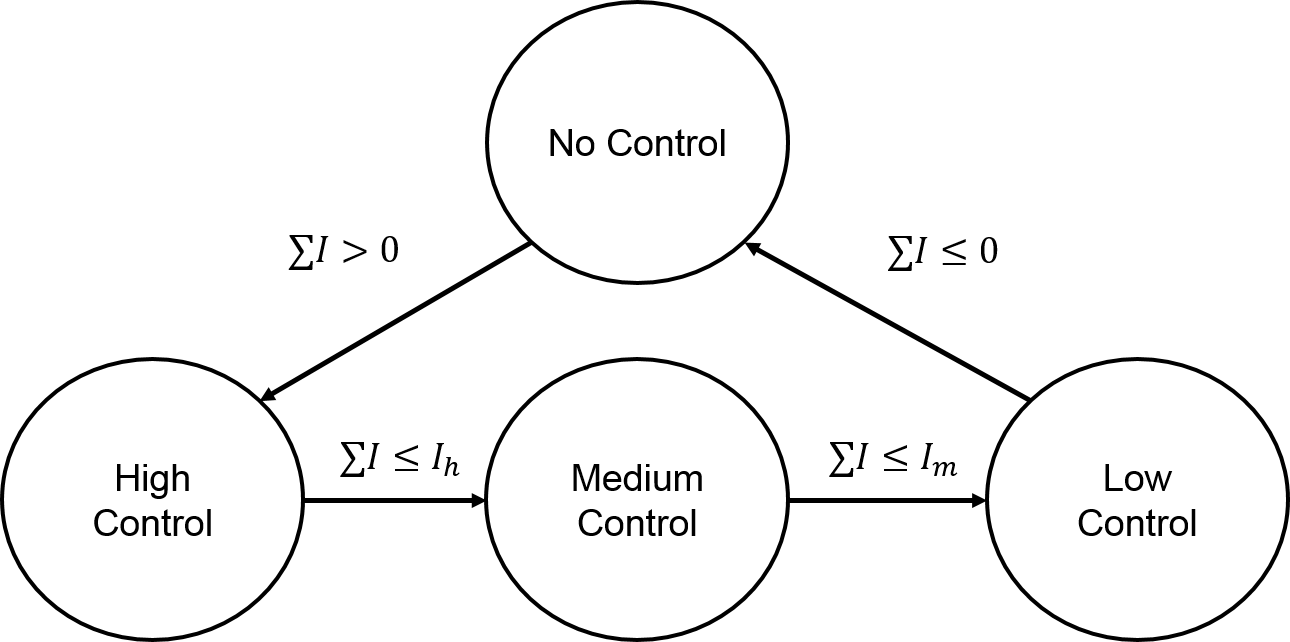
\includegraphics[width=100mm]{hybrid.png}
	\caption{Illustration of the hybrid system on controlling transportation system}
	\label{fig:hybrid}
\end{figure}

The transportation system dynamics may vary from no control to high control in the hybrid system, depending on the disease state in the network. The disease state can be considered as the guard condition for the hybrid system, where different amount of infected population may acquire different level of control on the traffic system. Intuitively, it is not efficient nor effective to place the highest level of control all the time. The hybrid system has a trivial reset, where the SEIR states remain the same upon mode switching, but the system dynamics differ. The system dynamics varies with different control strategies, where the utility theory will come into play. That is, when control is placed on transportation system, passengers' travel time will get affected and they will shift to other modes to maximize their utility. As a consequence, the disease dynamics and human contagion processes are also changed. 

As we have proved in the previous section, the DFE is only L.A.S. Therefore, the reachability analysis is necessary in order to evaluate if the DFE is reachable, and whether or not the hybrid transportation control system is effective. 

\section{Reachability Analysis}

As we have shown before, we build a hybrid system based on the transportation system with traffic control and there are four discrete modes in the hybrid system which correspond to three different control levels and no control case. Since our goal is to prevent disease from spreading by placing different levels of control on the transportation system, we want to compute the forward reachable sets of the hybrid system and their intersection with the unsafe set (e.g., $\sum R > 0.5N$) and determine whether the states will be driven towards the set of the first equilibrium points, i.e., the DFE. 

\subsection{Taylor model flowpipe construction}

We adopt the higher-order Taylor models (TM) in \cite{chen2012taylor} for the reachable set computation of non-linear hybrid systems.

A TM of order $k>0$ over domain $D\in \mathbb{I}^n$ is a pair $(p,I)$ of a polynomial $p$ of degree at most $k$ over $n$ variables $\vec{x}$ and remainder interval $I \in \mathbb{I}$. And $(p,I)$ is a k-order over-approximation of a function $f:D\mapsto \mathbb{R}$, denoted as $f\in (p,I)$. The arithmetic operations of TMs are similar to those of interval methods.

When integrating an ODE of the initial value problem (IVP) $\frac{d\vec{x}}{dt}=F(\vec{x},t)$ over the state $\vec{x}\in \mathbb{R}^n$, an initial interval $\vec{x}(0)\in X_0 \in \mathbb{I}^n$ for the values of $\vec{x}$ at time $0$ and a time interval $[t_1,t_2]\in \mathbb{I}$, where $X_0$ is the initial set and $\mathbb{I}$ is the set of all interval s in $\mathbb{R}$. And it is assumed that the ODE $F(\vec{x},t)$ is locally Lipshitz continuous, which ensures that the time trajectories exist and are unique over time interval $[-\Delta,\Delta]$ and $[t_1,t_2]\in [0,\Delta]$ with $\Delta \ge 0$. \par 

Based on these assumptions, the existence of a flow map $\vec{x}(t)=\varphi (\vec{x}_0,t)$ that maps a given initial condition $\vec{x}_0=\vec{x}_0$ to the state reached at time $t$. And it is possible to compute a TM $(p_k,I)$ of any given order $k\in \mathbb{N}$ for this map.\par 

Consider the ODE $\frac{d\vec{x}}{dt}=F(\vec{x},t)$ and a function $g(\vec{x}_0,t)$, the Picard operator defined by $F$ is 

\begin{equation}
\mathbb{P}_F(g)(\vec{x}_0,t)=\vec{x}_0+\int_0^t F(g(\vec{x}_0,s),s)\ ds 
\end{equation}

\noindent $\mathbb{P}_F$ is contractive and its unique fixed point defines the solution to the ODE if $F$ is Lipschitz continuous. And it can be applied to derive the Taylor expansion $p_n$ of order $n$ for its fixed point.


When using Lie derivatives of $\vec{x}(t)$ to compute the Taylor expansion for the flow map, it gives the value of the time derivative of the function $g(\vec{x}(t),t$ for any time trajectory $\vec{x}(t)$. The truncated series can be written as 

\begin{equation}
g_n(\vec{x}_0,t)=g(\vec{x}_0,0)+\mathcal{L}_F(g(\vec{x}_0,0))t+\mathcal{L}^2_F(g(\vec{x}_0,0))\frac{t^2}{2!}+\cdots+\mathcal{L}^n_F(g(\vec{x}_0,0))\frac{t^n}{n!}
\end{equation}

\noindent and apply the truncated Lie series for each function $f_j(\vec{x})=x_j$.

After computing a Taylor expansion $p_k$ of order $k$ for the flow map $\varphi$, we need to find a remainder interval to bound the error $e(\vec{x}_0,t)=\varphi(\vec{x}_0,t)-p_n(\vec{x}_0,t)$. A standard approach is as following:

\begin{enumerate}
\item Choose an initial interval $I_0$ based on estimation
\item Evaluate Picard operator over $p_k+I_0$ to get $(p'_k,I_1)$, where $I_1 \subseteq I_0$
\item Compute an enclosure of $p'_k-p_k+I_1$
\item If the enclosure is contained in $I_0$, stop, otherwise expand $I_0$ and repeat
\end{enumerate}

Hence, this process ensures that a flowpipe is generated that overapproximates the trajectories of the ODEs. And the forward reachable set is the union of all flowpipes across the time.

For hybrid systems, we need further to compute the intersection of TMs and guards of hybrid systems. And it is accomplished by domain contraction using interval constraint propagation (ICP).

Consider a TM flowpipe $S_j$: $(p_j(\vec{x}_0,t),I_j)$ over $\vec{x}_0\in D_0$, $t\in J$, and a guard set defined by predicate $\gamma (\vec{x})$. Then the intersection is 

\begin{equation}
\vec{x}=p_j(\vec{x}_0,t)+I_j \wedge \vec{x}_0\in D_0 \wedge t\in J \wedge \gamma(\vec{x})
\end{equation}

The constraint $\gamma(\vec{x})$ on the range will lead to a smaller domain $D'_0 \subseteq D_0$ for $\vec{x_0}$ and $J'\subseteq J$ for $t$, and a contracted TM $(p_j(\vec{x}_0,t),I_j)$, where $\vec{x}_0\in D'_0$, $t\in J'$. And the process of domain contraction using ICP is as following:

\begin{enumerate}
\item Define the original domain $D_0$ of interest in terms of $\vec{x}_0$ and $t$
\item Substitute $p_j(\vec{x}_0)+\vec{u}$ for $\vec{x}$ to express the constraint $\gamma(\vec{x})$ with $\vec{x}_0$ and $t$, where $\vec{u}$ represents uncertainty
\item Use ICP to contract $D_0$
\end{enumerate}

And this process can be improved by using branch-and-prune by partitioning the results from ICP into many small subsets and recursively applying ICP on each subset. The union of these results will give an improved contract domain.
 
\section{Numerical Results}
The numerical experiments are conducted on a desktop with @ 3.5 GHz CPU and $32GB$ RAM. The codes are written in C++ and compiled with g++ in Linux system. The MPFR library is used for interval arithmetic and the flow* library is used for doing TM model construction. 
We conduct the test on a 3-node network as shown in Figure~\ref{fig:network}.

\begin{figure}[h]
	\centering
	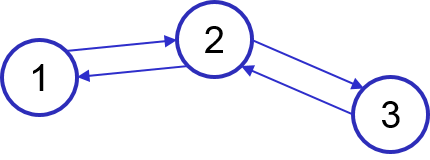
\includegraphics[width=50mm]{network.png}
	\caption{Test Network}
	\label{fig:network}
\end{figure}
The network results in 36 states variables and 36 system equations (9 travel pairs and 4 states: S,E,I,R for each pair). We consider the following initial conditions:
\begin{enumerate}
	\item $S_{11}=S_{12}=S_{13}\in[0.78,0.8]$, $I_{11}=I_{12}=I_{13}\in[0.18,0.2]$. All other $I=0$ and $S=1$. Therefore, there will be disease originated from zone $1$. 
	\item $t_0=0,t_{end}=20, \Delta t=0.1$. This results in 200 total steps. 
	\item For guards condition, we consider $I_h\leq 0.4$ and $I_m \leq 0.2$. As a result, we will start with High control mode since the total infected population is greater than 0.4. 
\end{enumerate}

The forward reachable set takes 954 seconds to complete for the 200 time steps. The results for the hybrid reachable set and its comparison with the no control case are presented in the following. 
\begin{figure}[H]
	\centering
	\subfloat[Hybrid $S_{11}$ versus $I_{11}$]{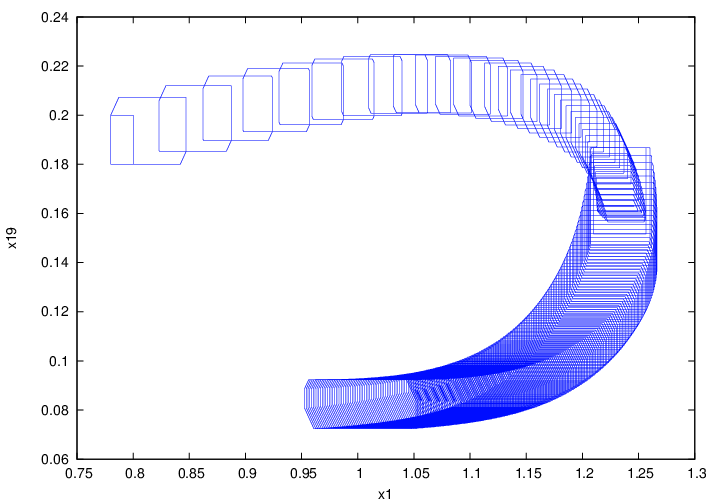
\includegraphics[width=80mm]{results/images/hb_x1_x19.png}}
	\subfloat[No control $S_{12}$ versus $I_{12}$]{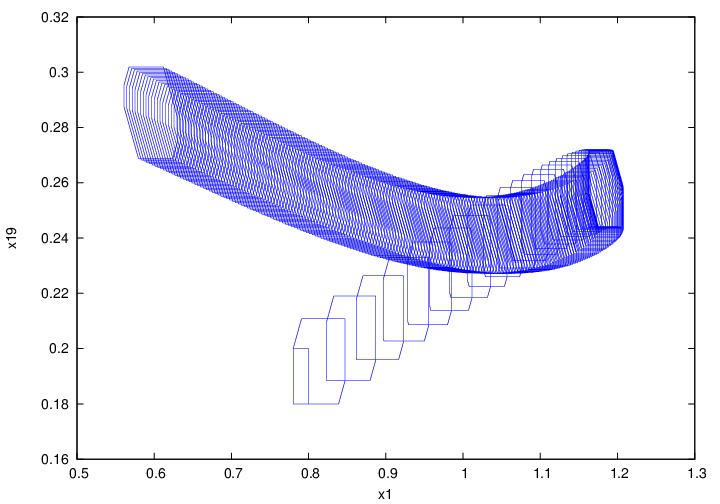
\includegraphics[width=80mm]{results/images/sg_x1_x19.png}}\\
	\subfloat[Hybrid $S_{12}$ versus $I_{12}$]{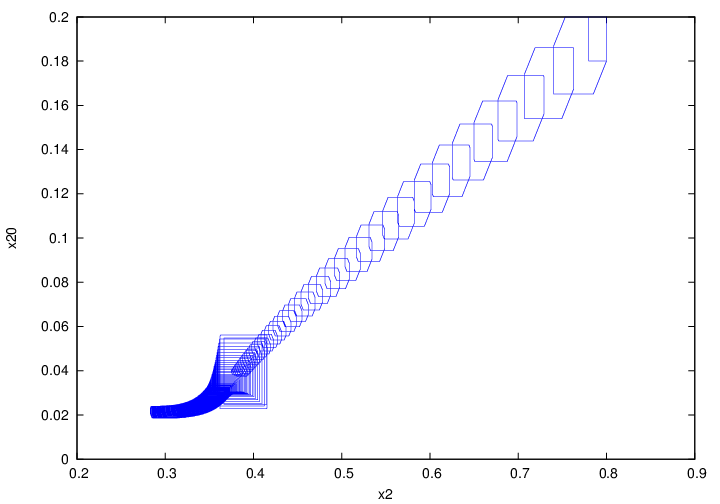
\includegraphics[width=80mm]{results/images/hb_x2_x20.png}}
	\subfloat[No Control $S_{11}$ versus $I_{11}$]{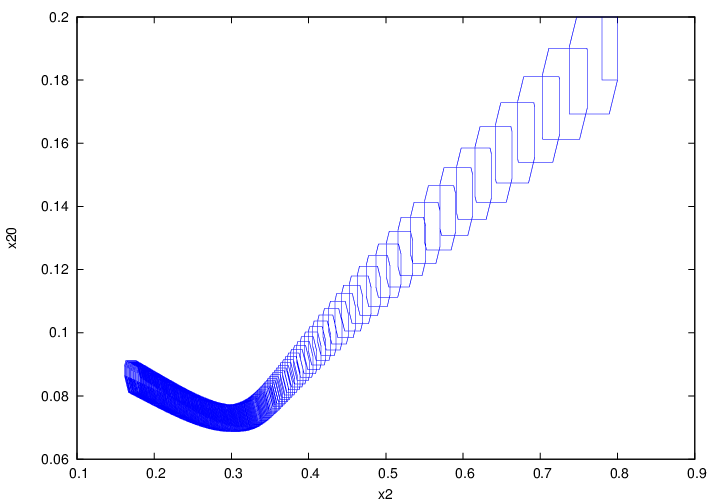
\includegraphics[width=80mm]{results/images/sg_x2_x20.png}}\\
	\subfloat[Hybrid $S_{33}$ versus $I_{33}$]{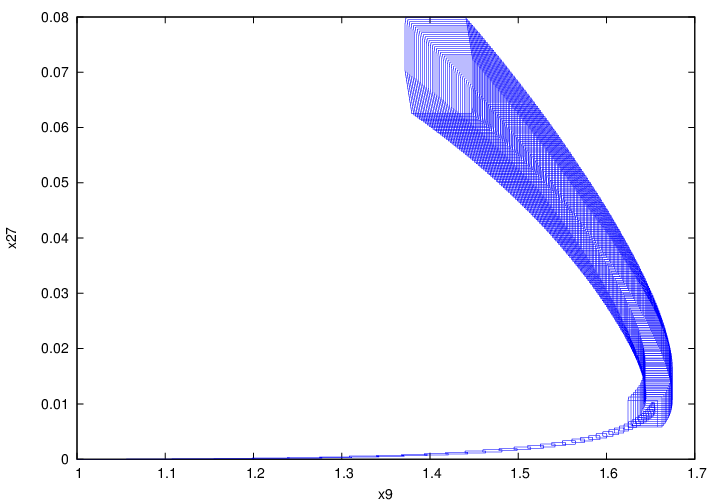
\includegraphics[width=80mm]{results/images/hb_x9_x27.png}}
	\subfloat[No Control $S_{11}$ versus $I_{11}$]{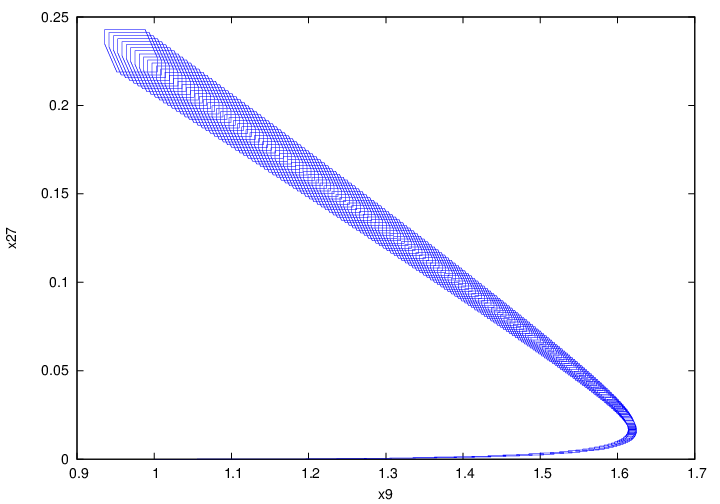
\includegraphics[width=80mm]{results/images/sg_x9_x27.png}}
	\caption{Comparison of no-control scheme versus hybrid system setting}
	\label{fig:compare}
\end{figure}

For Figure~\ref{fig:compare} (a)-(d), they show the reachable set when starting from the infected states, where the infected population $\in[0.18,0.2]$. It can be verified that the traffic control does help to eliminate the disease and reduce the spread of the disease. In particular, for $I_{11}$, it can be seen that at the end of the time interval the infected population is reduced to $[0.07,0.09]$, while for the no control case there is a clear sign of disease outbreak since there are 50\% more infected people. Similarly, for $I_{12}$, the control helps to reduce the infected population to less than $0.02$, and the overall trend is monotonically decreasing, but the no control case has a larger population of infectious people and the amount of infected people increases towards the end. As for $I_{33}$, it starts from the DFE state, and the no control case clearly shows the pattern of disease outbreak, while for the controlled system there are much fewer infected population. Also, the amount of infected people tends to decrease if we enlarge the time interval. 

 
\bibliographystyle{unsrt}
\bibliography{main}
\end{document}